\chapter{\textit{Grasp}について}
\label{graspについて}

第\ref{related_works}章では、「身体化」に関する先行研究について、それぞれの分野でどのように展開しているのかについてを概観し、その中での本研究の位置付けと貢献を示した。

本章では、本研究における「人馬一体」といった関係性についてより詳細に捉えるため、Sydney Felsによるembodimentの分類を導入する。
そして、身体化過程における意識的な試行期間を捉える新たな概念として\textit{grasp}を提示する。その上で、Felsの分類との関係性と、この概念を用いることから修士作品の体験についてのねらいを説明する。また、この概念に至るまでのプロトタイピングの過程を示すことで、この概念を主張する根拠とする。

\section{Felsのembodiment}
コンピューター工学の研究者であるSydney Felsは2000年、「Intimacy and Embodiment: Implications for Art and Technology」\cite{Fels}において、人間と対象との関係性を「embodiment」の観点から4つのカテゴリに分類した。
それぞれの説明は以下の通りである(括弧内は筆者訳)。

\textbf{Response(応答):}\\
対象に対する作用の結果から、感情的な反応や理解を得る状態を指す。Felsはこの関係性の例として「コンピュータとそれに初めて触れた人」を挙げ、「なんらかの操作を通して得られた、便利な機能に喜んでいる状態、また逆に「有用な結果を得られず落胆する状態」と説明する。

\textbf{Control(制御):}\\
人が対象を自分自身の延長として使用し、その操作によって感情的な満足や美的体験を得る状態を指す。例えばピアノの演奏において、「音が出ている」ということだけでなく、自分自身の表現したいことが、不自由なくピアノを通して体現されていると感じるときの、一体感によってもたらされる心地よさがこれに該当する\footnote{「Control」においてFelsは、「自分自身の延長」として経験される感覚であり、またそれが追従性の高いグラフィックによってもたらされると説明する。これは、渡邊がマウスカーソルやスマートフォンに対して用いた「操作時の指とグラフィックの追従性が高い」インターフェースという説明と同等のものであると考えられる。このことからFelsの分類におけるControlは、渡邊の「自己帰属感」と重なる。}。

\textbf{Contemplation(鑑賞):}\\
人が対象に対して働きかけることはないが、人がその対象からの信号やメッセージを内省や反映を通じて、感情的になったり美的体験を得る状態を指す。Felsはその具体例として、絵画の鑑賞体験を挙げる。

\textbf{Belonging(帰属):}\\
対象によって人が動かされているような経験を指す。人はその対象によって提供される体験を通じて感情的な反応を得る。ここでは、対象が人の体験や感情を形作る役割を果たす。たとえばバイクの運転において、「バイクに合わせた走り方をする」といったように、単にその対象を通して使い手の意図がそのまま体現されるのではなく、その対象に合わせた振る舞いがそこで形作られることに喜びを見出すような状態である。

\begin{figure}[H]
  \centering
  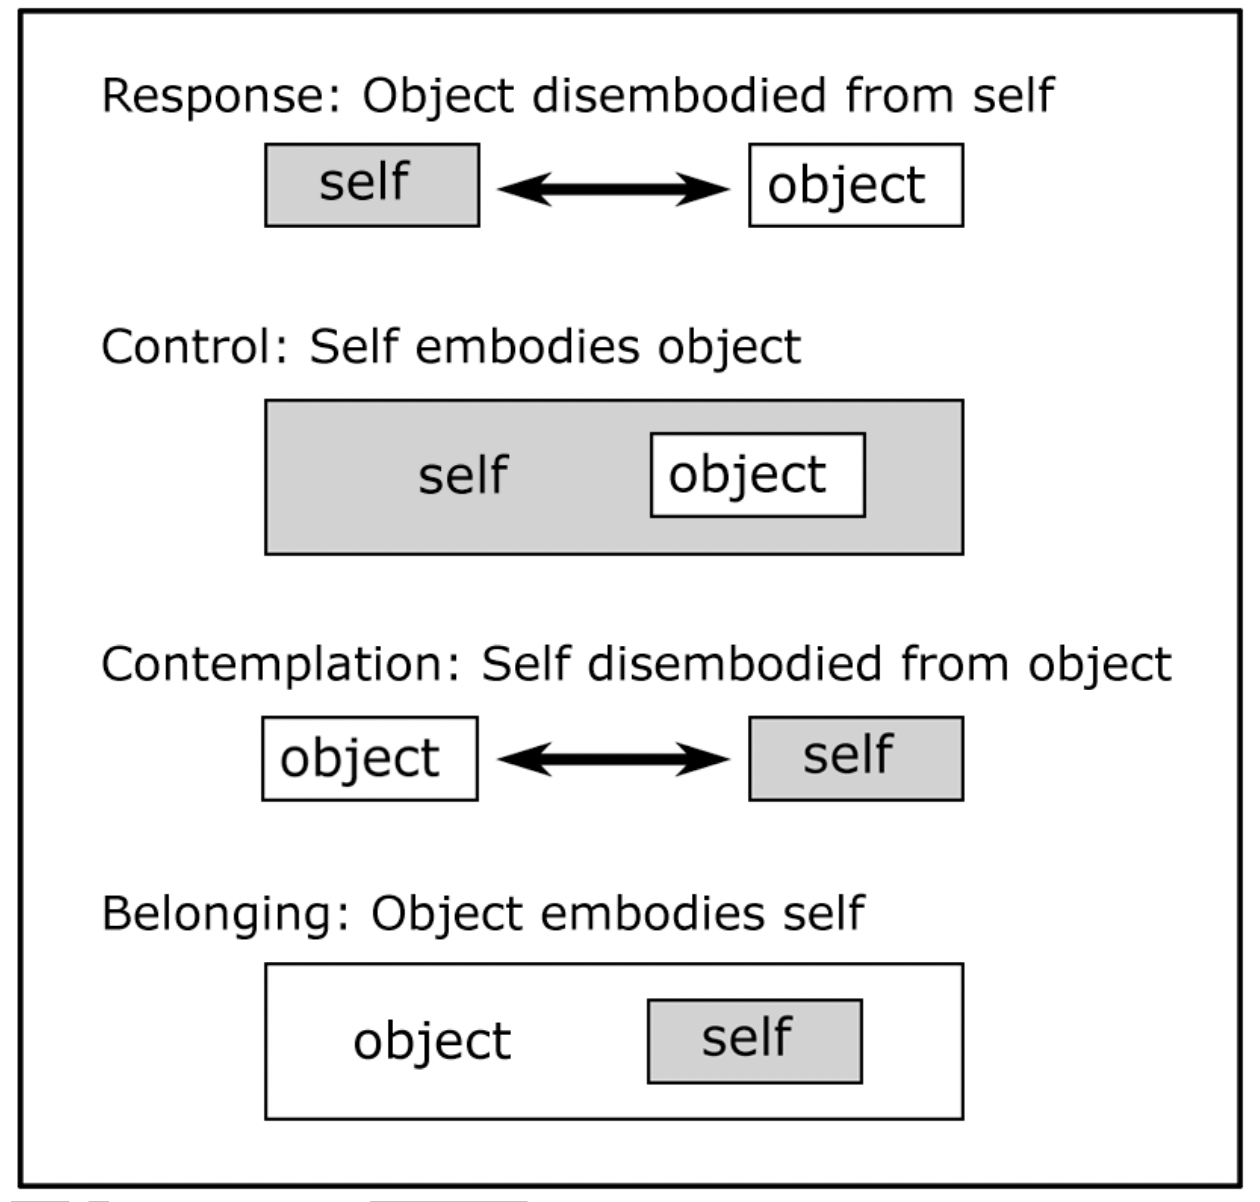
\includegraphics[width=8cm]{img/fels_diagram.png}
  \caption{Felsによるembodiment(仮置き)}
  \label{fig:fels_embodiment}
\end{figure}

% さて、Felsは特に、上記「制御 Control」においては「自分自身の延長」として経験される感覚について言及しており、またそれが追従性の高いグラフィックによってもたらされるという記述は、渡邊がマウスカーソルやスマートフォンに対して用いた「操作時の指とグラフィックの追従性が高い」インターフェースという説明と同等のものである。このことからFelsのいうControlとは、Gallagherの「sense of ownership」と同じものを指していると考えられる。その上で、embodimentの状態をControlのみならずBelongingから捉えていること、そしてembodimentが生じていない状態についても言及していることなど、現在HCIの分野で一般に用いられる意味でのembodimentよりも広く、人と対象を捉えるモデルとなっていることが確認できる。

% さらにFelsは、対象と人とのあいだにある「深い関係」を指して、「Intimacy」という尺度で説明する。例えば楽器と人の関係性ように、Intimacyのある関係性のもとでは、「あたかもその装置が身体の延長であるかのように、考えや感情を効果的に表現できる」という。上記の、Felsによるembodimentの分類においては、ResponseがIntimacyの低い状態、ControlがIntimacyの高い状態として説明される。

他者性と向き合う中で、自分なりの扱い方を見出すことは、Felsの分類における「Belonging」であると言える。しかしこの状態であっても、「Control」も同時に行われている。またFelsは、自分の意志と対象の制約や他者性とのあいだで折り合いをつけることで得られる「親密な関係」を、「Intimacy」という言葉で説明した\footnote{"\textit{Intimacy deals with the subjective match between the behaviour of a device and the operation of that device.}"Fels(2000)\cite{Fels}より}。

このことから、本研究が目指す「人馬一体」という言葉をFelsの用語を用いると、
\begin{quote}
  「Control」と「Belonging」が両方生起することで生じる「Intimacy」
\end{quote}
と説明できる。しかし、Felsはこうした分類を行ったが、それらがどのようにして生起するかについては述べていない。そこで、本研究では次節に定義する\textit{grasp}こそが、その生起に重要な役割を果たしているのではないかという仮説を立てた。


\section{\textit{grasp}の定義}
\label{grasp_difinition}
\textit{grasp}について、本研究では次のように定義する。

\begin{quote}
  \textbf{人と対象との関係の中で、人が対象の中に注意や目的意識を抱きながら、意識的に試行する期間}
\end{quote}

graspは「把握」を意味する動詞でもあるが、ここで「動作」ではなく「期間」とした。その理由は、「意識的に試行する」とき、同時にその結果を受けて気づきを得たり、その気づきをもとに新たな関心を抱くといった、単に自分が行為しているだけではなく、対象から影響を受けながら次の行為が決まってくるようなフィードバックループの構造があると考えるためである。「grasp=把握」という言葉についても、単に「ものを掴む」という意味だけでなく、「理解」の意味があることは、対象について一方向に働きかけているのではない様子が現れているのではないだろうか。

\textit{grasp}とは例えば、ギターの習得過程において、弾きこなしたいフレーズを定め、それを達成するまでに試行錯誤をし、達成できるようになるまでの期間である。熟達した状態では、熟達する前とは違う視座でものごとを捉えられるようになり、また違う対象に注意が向くようになると、ギターと人との間に別の\textit{grasp}が芽生える。
またあるいは、\textit{grasp}の過程で、対象と向き合い続ける過程の中でその解像度が高まり、当初目指していたこととは違うことに興味を抱く(セレンディピティ)ことでも、別の\textit{grasp}が芽生える。

ここまで具体例を通してみてきたように、\textit{grasp}は、ギターと人との関係において一度だけ生じるのではなく、注目する対象が定まれば何度でも生じる。
% ここで、\textit{grasp}は人と対象の関係の中で、人が注意を向ける「対象」ごとに別の\textit{grasp}があると言えそうだが、注意を向けている「対象」がなんであるか、断言できなかったり、本人も判然としないこともある。そのため、


\section{Felsの議論との関係性}
ここでは\textit{grasp}が、FelsのEmbodimentとどう関係するのかについて説明する。
\ref{grasp_difinition}節に挙げたように、\textit{grasp}の中で、対象から影響を受けながら次の試行が形作られていくと考える。この時の「試行」には、挙動を確かめるような動作、すなわちFelsの「Response」もあれば、試行を通して得られた結果をもとに、何かに考えを巡らす「Contemplation」も含まれる。こうした試行の積み重なりから、人と対象のあいだに「Control」や「Belonging」の関係、すなわちFelsの意味でのIntimacyが生じるのではないか。

\section{\textit{grasp}を踏まえたIntimacyが起こるまでの過程についての仮説}
\textit{grasp}が、本研究の関心である「「Control」と「Belonging」が両方生起することで生じる「Intimacy」」までの過程に必要ではないか、と考える。

% そしてそのためには、注意を向ける対象や目的意識を抱く対象が変わりながらも\textit{grasp}が継続していく体験が良いのか、それとも注意を向ける対象は変わらず、1つのものに対する目的意識が長く継続し、\textit{grasp}も長い体験が良いのか。このいずれであるかが判別することができれば、より詳細にこの体験を説明することができると考えた。